\documentclass{article}
\usepackage{amsmath}
\usepackage{physics}
\usepackage{amssymb}
\usepackage[UTF8, fontset=none]{ctex} % 禁用默认字体
\usepackage{fontspec}
\usepackage{graphicx}
\setmainfont{Noto Sans CJK SC}
\title{脏图生成的数学原理推导}
\author{}
\date{}

\begin{document}
\maketitle

\section{可见度与天空亮度的关系}
综合孔径干涉测量中,可见度函数 $ V(u,v) $ 是天空亮度分布 $ I(l,m) $ 的二维傅里叶变换。设方向余弦 $ (l,m) $ 对应天空坐标,空间频率 $ (u,v) $ 对应基线在赤道面的投影(以波长为单位),则有:

\begin{equation}
V(u,v) = \iint I(l,m) e^{-2\pi i (ul + vm)} \, dl \, dm
\label{eq:fourier}
\end{equation}

其逆变换为:
\begin{equation}
I_{\text{dirty}}(l,m) = \iint V(u,v) e^{2\pi i (ul + vm)} \, du \, dv
\label{eq:inv_fourier}
\end{equation}

\section{非完备采样与脏束}
实际观测中,$ V(u,v) $ 仅在离散位置 $ \{(u_k,v_k)\} $ 处采样。定义采样函数:
\begin{equation}
S(u,v) = \sum_{k} \delta(u - u_k) \delta(v - v_k)
\end{equation}

观测的可见度数据为:
\begin{equation}
V_{\text{obs}}(u,v) = V(u,v) \cdot S(u,v)
\end{equation}

代入逆变换公式,脏图可表示为:
\begin{equation}
I_{\text{dirty}}(l,m) = I(l,m) \ast B(l,m)
\end{equation}

其中 $ B(l,m) $ 是脏束(点扩散函数),满足:
\begin{equation}
B(l,m) = \iint S(u,v) e^{2\pi i (ul + vm)} \, du \, dv
\label{eq:dirty_beam}
\end{equation}

\section{网格化与离散傅里叶变换}
为使用快速算法(FFT),需将非均匀采样的可见度数据映射到均匀网格。设网格间距为 $ \Delta u, \Delta v $,网格点数为 $ N \times N $,则:

\subsection{最近邻网格化}
将每个可见度点 $ (u_k,v_k) $ 分配到最近的网格位置:
\begin{equation}
i_k = \text{round}\left( \frac{u_k}{\Delta u} + \frac{N}{2} \right), \quad j_k = \text{round}\left( \frac{v_k}{\Delta v} + \frac{N}{2} \right)
\end{equation}

网格化后的可见度矩阵为:
\begin{equation}
\widetilde{V}[i,j] = \sum_{k} V_k \cdot \delta(i - i_k) \delta(j - j_k)
\end{equation}

\subsection{逆离散傅里叶变换}
脏图通过逆 FFT 计算:
\begin{equation}
I_{\text{dirty}}[p,q] = \frac{1}{N^2} \sum_{i=0}^{N-1} \sum_{j=0}^{N-1} \widetilde{V}[i,j] e^{2\pi i (pi/N + qj/N)}
\end{equation}

\section{坐标缩放与平移}
为正确显示天空方向余弦 $ (l,m) \in [-0.5, 0.5] $,需引入缩放因子 $ \alpha $ 和平移操作:

\subsection{缩放}
设最大空间频率为 $ u_{\max} $,则缩放因子为:
\begin{equation}
\alpha = \frac{N/2}{u_{\max}}
\end{equation}

缩放后的坐标为:
\begin{equation}
\tilde{u}_k = \alpha u_k, \quad \tilde{v}_k = \alpha v_k
\end{equation}

\subsection{平移}
将 FFT 的坐标原点移至图像中心:
\begin{equation}
\widetilde{V}_{\text{shift}}[i,j] = \widetilde{V} \left[ (i + N/2) \bmod N, (j + N/2) \bmod N \right]
\end{equation}

最终脏图的像素坐标 $ (p,q) $ 对应方向余弦:
\begin{equation}
l_p = \frac{p - N/2}{\alpha N}, \quad m_q = \frac{q - N/2}{\alpha N}
\end{equation}

\section{结论}
脏图生成的核心步骤可总结为:
\begin{align}
I_{\text{dirty}} &= \mathcal{F}^{-1} \left[ S) \cdot V(u,v) \right] \\
&= I(l,m) \ast B(l,m)
\end{align}

其中网格化和坐标变换保证了离散计算与连续理论的等价性。

\section{结果}
    \begin{figure}[htp]
    \centering
    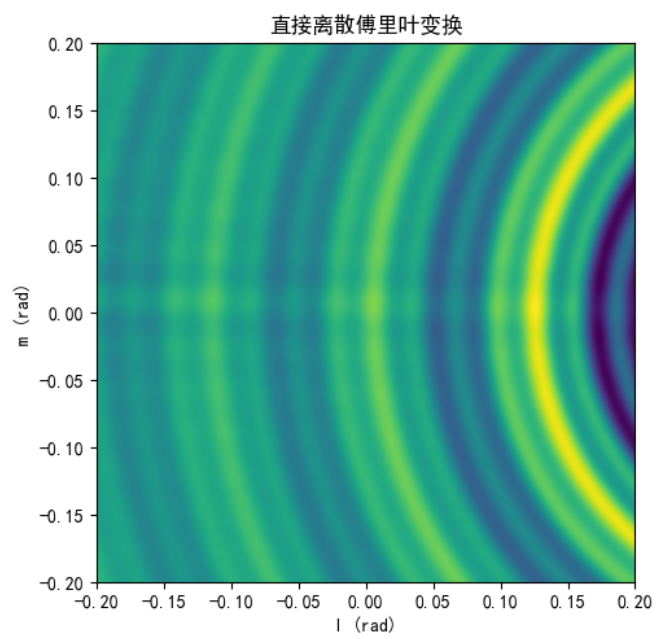
\includegraphics[width=1\textwidth]{task4/task4_fft_dirty.png}
    \label{fig:fft}
    \end{figure}
    
    \begin{figure}[htp]
    \centering
    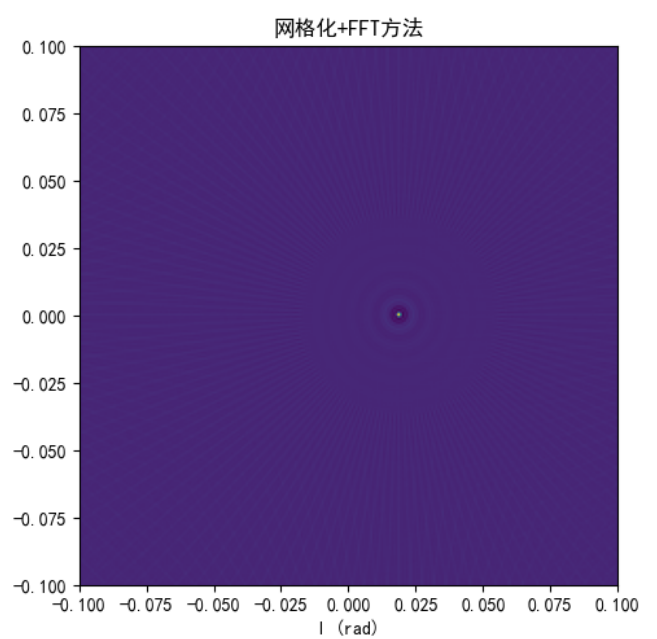
\includegraphics[width=1\textwidth]{task4/task4_gridfft_dirty.png}
    \label{fig:gridfft}
    \end{figure}
\end{document}